\documentclass[10pt]{beamer}

% ======================
% Pacotes básicos
% ======================
\usepackage[utf8]{inputenc}
\usepackage[T1]{fontenc}
\usepackage[provide=*,main=portuguese]{babel}
\usepackage{amsmath, amsfonts, amssymb}
\usepackage{graphicx}
\usepackage{booktabs}
\usepackage{xcolor}
\usepackage{array}
\usepackage{tabularx}
\usepackage{tikz}
\usetikzlibrary{positioning,arrows.meta}

\usetheme{Madrid}

% ======================
% Infos da capa
% ======================
\title[seqKAN - Resultados]{seqKAN - Resultados de Treino}
\author{Fernanda Mickosz Villa Verde}
\institute{CPE-883 - Aprendizado de Máquina}
\date{\today}

\begin{document}

\begin{frame}
  \titlepage
\end{frame}

\begin{frame}{Sumário}
\tableofcontents
\end{frame}

\section{Resumo}
\begin{frame}{Resumo}
\begin{itemize}
\item Objetivo: avaliar o modelo seqKAN para reconstrução de séries temporais industriais buscando maior interpretação.
\item seqKAN: modelo baseado em splines B-spline para modelar relações não lineares e temporais.
\item Metodologia: treino supervisionado com loss de reconstrução, usando métricas MSE e SE.
\end{itemize}
\end{frame}

\section{Metodologia}
\begin{frame}{Metodologia}
\begin{itemize}
\item Modelo: seqKAN com m\'ultiplos blocos KAN (kan\_x, kan\_h, kan\_zx, kan\_zz, kan\_out) e parte recorrente.
\item Parte recorrente: atualiza\c{c}\~ao temporal de estados $h_t$ e $z_t$ (dependem de $t-1$).
\item Treino supervisionado com reconstrução e sem regularização.
\item Métricas: MSE e SE (macro e micro).
\end{itemize}
\end{frame}

\begin{frame}{Metodologia: Fórmulas do seqKAN (I)}
\begin{itemize}
\item Base B-spline (Cox--de Boor):
\end{itemize}
\vspace{-0.5em}
\[
\begin{aligned}
B_{i,0}(x) &= \mathbb{1}_{[t_i,\, t_{i+1})}(x) \\
B_{i,k}(x) &= \frac{x-t_i}{t_{i+k}-t_i} B_{i,k-1}(x) + \frac{t_{i+k+1}-x}{t_{i+k+1}-t_{i+1}} B_{i+1,k-1}(x)
\end{aligned}
\]
\begin{itemize}
\item \texttt{coef2curve} (por batch, input e output):
\end{itemize}
\vspace{-0.5em}
\[
 y_{b,i,j} = \sum_{m} B_{b,i,m}(x)\, c_{i,j,m}
\]
\end{frame}

\begin{frame}{Metodologia: Fórmulas do seqKAN (II)}
\begin{itemize}
\item Sa\'ida da camada (\texttt{KANLayer}):
\end{itemize}
\vspace{-0.5em}
\[
\hat{y}_{b,j} = \sum_{i} m_{i,j}\, y_{b,i,j}
\]
\begin{itemize}
\item Sa\'ida spline aplicada \`a entrada: $s_1(x_t)=\mathrm{KAN}_x(x_t)$, com
\end{itemize}
\vspace{-0.5em}
\[
 y_{b,i,j} = \sum_{m} B_{b,i,m}(x_t)\, c_{i,j,m}, \qquad
 s_{1,b,j} = \sum_{i} m_{i,j}\, y_{b,i,j}
\]

\begin{itemize}
\item F\'ormula geral da KAN (sa\'ida $j$):
\end{itemize}
\vspace{-0.5em}
\[
\mathrm{KAN}_j(x) = \sum_{i} m_{i,j} \sum_{m} c_{i,j,m}\, B_{i,m}(x_i)
\]

\end{frame}



\begin{frame}{Metodologia: Loss de Reconstru\c{c}\~ao}
\begin{itemize}
\item Loss (L1): soma do erro ao quadrado com m\'ascara, normalizada pelo n\'umero de observa\c{c}\~oes.
\end{itemize}
\vspace{-0.5em}
\[
\mathrm{SSE}_{b,t} = \sum_{d} (x_{b,t,d} - \hat{x}_{b,t,d})^2 \cdot \mathrm{mask}_{b,t,d} \cdot c_{b,t,d}
\]
\[
\mathrm{nobs}_{b,t} = \sum_{d} \mathrm{mask}_{b,t,d} \cdot c_{b,t,d}
\]
\[
\mathcal{L}_{rec} = \frac{\sum_{b,t} \mathrm{SSE}_{b,t}}{\sum_{b,t} \mathrm{nobs}_{b,t}}
\]
\begin{itemize}
\item Observa\c{c}\~oes ausentes n\~ao contribuem (m\'ascara).
\end{itemize}
\end{frame}



\begin{frame}{Metodologia: Din\^amica Paralela}
\begin{equation*}
 h_t = h_{t-1} + m \cdot s_1(x_t) + (1-m) \cdot z_{t-1}
\end{equation*}
\begin{itemize}
\item $h_t$: estado oculto principal no tempo $t$.
\item $s_1(x_t)$: sa\'ida spline (seqKAN) aplicada \`a entrada $x_t$.
\item $z_{t-1}$: estado de uma seqKAN paralela, adiciona uma \textbf{segunda mem\'oria recorrente} (especialmente quando falta dado).
\item $m$: gate derivado de \texttt{mask}. Se \texttt{mask=None}, $m=1$ (s\'o caminho principal).
\item Se \texttt{mask} indica falta de dado em $t$, $m$ tende a 0, privilegiando o caminho paralelo.
\item Se \texttt{mask} n\~ao tem tamanho $H$, o gate vira um \textbf{escalar por amostra} (mesmo $m$ para todos os neur\^onios). Se tem tamanho $H$, o gate \`e um \textbf{vetor por hidden}.
\end{itemize}
\end{frame}


\begin{frame}{Spline Aux Residual na Saída}
\small
\textbf{Intenção:} Corrigir comportamento nos extremos (cauda), mantendo a região central inalterada.

\textbf{Caminho paralelo com $z_{t-1}$:}
No modelo base, o caminho paralelo com $z_{t-1}$ atua \emph{dentro} da dinâmica do estado:
$h_t \leftarrow h_{t-1} + m\,\mathrm{KAN}_x(x_t) + (1-m)\,z_{t-1}$.
Ou seja, $z_{t-1}$ é uma segunda memória recorrente que interfere na atualização de $h_t$.

\textbf{Spline Aux residual na saída:}
A AuxSpline atua \emph{fora} da dinâmica: ela adiciona um \emph{corretor direto na saída},
somando um resíduo $\Delta y_t$ calculado a partir de $x_t$, sem alterar $h_t$.

\textbf{Residual na saída:}
$y_t=\mathrm{KAN}_{out}(h_t) + \alpha\,g(x_t)\,\mathrm{KAN}^{aux}_{out}(x_t)$,
com gate ativando o resíduo apenas fora da faixa nominal:
$g=\sigma(\alpha_x(|x_t|-2))$.


\end{frame}



\begin{frame}{Diagrama da Arquitetura}
\centering
\small
\resizebox{\textwidth}{!}{%
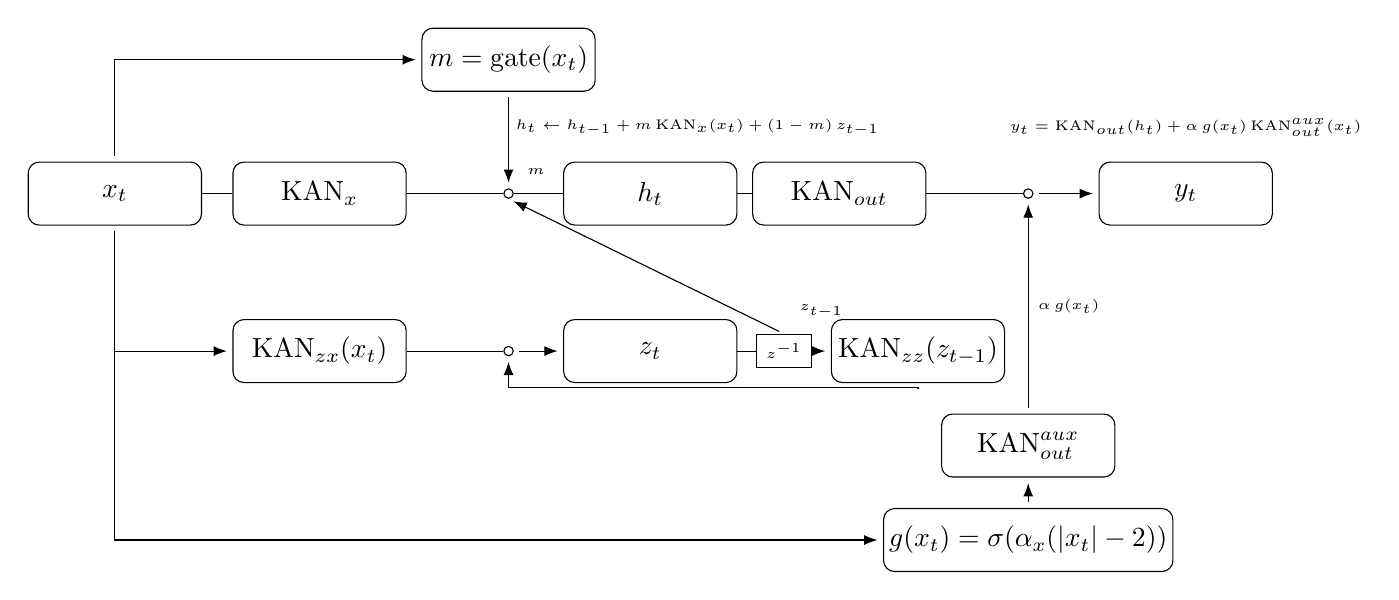
\begin{tikzpicture}[
  box/.style={draw, rounded corners, align=center, minimum width=22mm, minimum height=8mm, inner sep=2pt},
  sum/.style={draw, circle, inner sep=1.2pt},
  arrow/.style={-Latex, shorten >=2pt, shorten <=2pt}
]
  % Coordenadas fixas para evitar cruzamentos
  \node[box] (x)      at (0, 0) {$x_t$};
  \node[box] (kanx)   at (2.6, 0) {$\mathrm{KAN}_x$};
  \node[sum] (sumh)   at (5.0, 0) {};
  \node[box] (h)      at (6.8, 0) {$h_t$};
  \node[box] (kanout) at (9.2, 0) {$\mathrm{KAN}_{out}$};
  \node[sum] (sumy)   at (11.6, 0) {};
  \node[box] (y)      at (13.6, 0) {$y_t$};

  % Linha paralela (z)
  \node[box] (kanzx)  at (2.6, -2.0) {$\mathrm{KAN}_{zx}(x_t)$};
  \node[sum] (sumz)   at (5.0, -2.0) {};
  \node[box] (z)      at (6.8, -2.0) {$z_t$};
  \node[box] (kanzz)  at (10.2, -2.0) {$\mathrm{KAN}_{zz}(z_{t-1})$};

  % Gate e aux
  \node[box] (gate)   at (5.0, 1.7) {$m=\mathrm{gate}(x_t)$};
  \node[box] (aux)    at (11.6, -3.2) {$\mathrm{KAN}^{aux}_{out}$};
  \node[box] (gaux)   at (11.6, -4.4) {$g(x_t)=\sigma(\alpha_x(|x_t|-2))$};

  % Linha principal
  \draw[arrow] (x) -- (kanx) -- (sumh) -- (h) -- (kanout) -- (sumy) -- (y);

  % Linha z (sem cruzar caixas)
  \draw[arrow] (x.south) |- (kanzx.west);
  \draw[arrow] (kanzx) -- (sumz) -- (z);
  \node[draw, minimum width=7mm, minimum height=4mm, font=\tiny] (zdelay) at (8.5, -2.0) {$z^{-1}$};
  \draw[arrow] (z) -- (zdelay) -- node[midway, above, yshift=3mm] {\tiny $z_{t-1}$} (kanzz);
  \draw[arrow] (kanzz.south) |- ([yshift=-4mm]sumz.south) -- (sumz.south);
  \draw[arrow] (zdelay.north) -- (sumh.south);

  % Gate
  \draw[arrow] (x.north) -- ++(0,0.6) |- (gate.west);
  \draw[arrow] (gate) -- (sumh);
  \node[above right=1mm of sumh] {\tiny $m$};

  % Aux residual
  \draw[arrow] (x.south) |- (gaux.west);
  \draw[arrow] (gaux.north) -- (aux.south);
  \draw[arrow] (aux.north) -- (sumy.south) node[midway, right] {\tiny $\alpha\,g(x_t)$};

  % Labels
  \node[above=2mm of h, xshift=6mm] {\tiny $h_t \leftarrow h_{t-1} + m\,\mathrm{KAN}_x(x_t) + (1-m)\,z_{t-1}$};
  \node[above=2mm of y] {\tiny $y_t=\mathrm{KAN}_{out}(h_t) + \alpha\,g(x_t)\,\mathrm{KAN}^{aux}_{out}(x_t)$};
\end{tikzpicture}
}
\end{frame}

\section{Experimentos}
\begin{frame}{Experimentos}
\begin{itemize}
\item Dataset: séries temporais industriais (Cognite).
\item Divisão: janelas temporais com janela fixa e passo fixo.
\item Avaliação: métricas agregadas e por grupo (classes 0 e 1).
\end{itemize}
\end{frame}

\section{Resultados}
\begin{frame}{Resultados Globais}
\centering
\begin{table}
\centering
\caption{Comparação dos experimentos seqKAN (L1 e MSE micro)}
\resizebox{\linewidth}{!}{%
\begin{tabular}{l r r r}
\toprule
Run & L1 (ult. época) & Micro ($\mu \pm \sigma$) & Tempo (min) \\
\midrule
GRU Difusão      & - & $0.237 \pm 0.064$ & 10.1\\
Grid 40 Clamp-6/6 RAdam + AuxSpline (grid12, gate $|x|{-}2$) &  &  & \\
Grid 40 Clamp-6/6 RAdam + AuxSpline (grid12, gate $|x|{-}2$) & 0.331 & 0.239 ± 0.007 & 11.2\\
Grid 40 Clamp-6/6 RAdam & 0.390 & $0.269 \pm 0.006$ & 9.3 \\
Grid 40 Clamp-6/6 Adam  & 0.391 & $0.274 \pm 0.007$ & 8.6\\
Grid 40 Clamp-10/10 Adam & 0.464 & $0.286 \pm 0.009$ & 9.1 \\
Grid 20 Clamp-10/10 Adam & 0.499 & $0.300 \pm 0.009$ & 7.9\\
\bottomrule
\end{tabular}}
\end{table}


\end{frame}

\begin{frame}{Resultados por Grupo}
\centering

\begin{table}[H]
\centering
\caption{Resultados por grupos}
\label{tab:seqkan_pergroup_3runs}
\resizebox{\linewidth}{!}{%
\begin{tabular}{l c c}
\toprule
Run & Grupo 0 ($\mu \pm \sigma$) & Grupo 1 ($\mu \pm \sigma$) \\
\midrule
Grid 40 Clamp-6/6 RAdam + AuxSpline (grid12, gate $|x|{-}2$) &    & \\
Grid 40 Clamp-6/6 RAdam + AuxSpline (grid12, gate $|x|{-}2$)   &  0.208 ± 0.004 &  0.525 ± 0.049 \\
Grid 40 Clamp-6/6 RAdam  & $0.237 \pm 0.005$ & $\mathbf{0.563 \pm 0.046}$ \\
Grid 40 Clamp-6/6 Adam   & $\mathbf{0.238 \pm 0.005}$ & $\mathbf{0.606 \pm 0.059}$ \\
Grid 40 Clamp-10/10 Adam & $0.242 \pm 0.005$      & $0.681 \pm 0.074$ \\
Grid 20 Clamp-10/10 Adam & $0.257 \pm 0.005$ & $0.683 \pm 0.078$ \\
\bottomrule
\end{tabular}}
\end{table}
\end{frame}



\begin{frame}{Resultados - Gráficos por Run}
\centering
\setlength{\tabcolsep}{2pt}
\begin{tabular}{ccc}
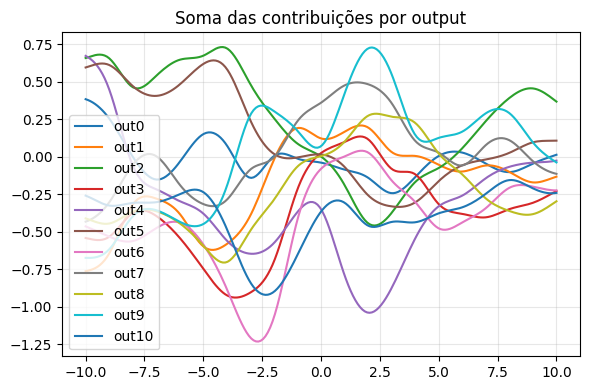
\includegraphics[width=0.28\linewidth]{../output20-1010.png} &
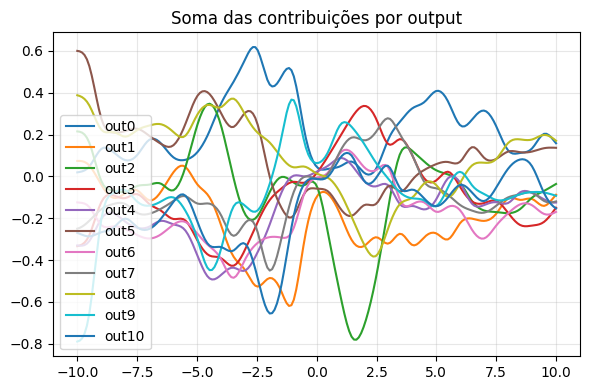
\includegraphics[width=0.28\linewidth]{../output40-1010.png} &
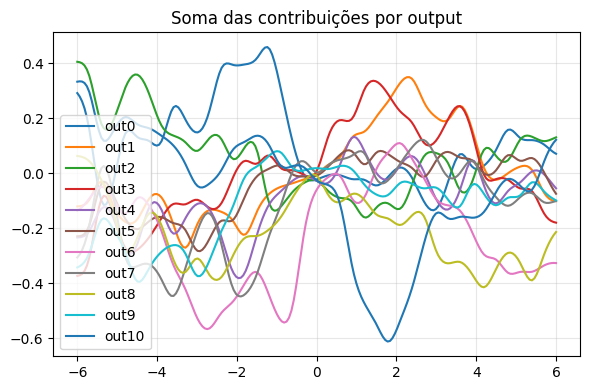
\includegraphics[width=0.28\linewidth]{../output40-66.png} \\
\tiny Grid 20 Clamp-10/10 Adam &
\tiny Grid 40 Clamp-10/10 Adam &
\tiny Grid 40 Clamp-6/6 Adam \\
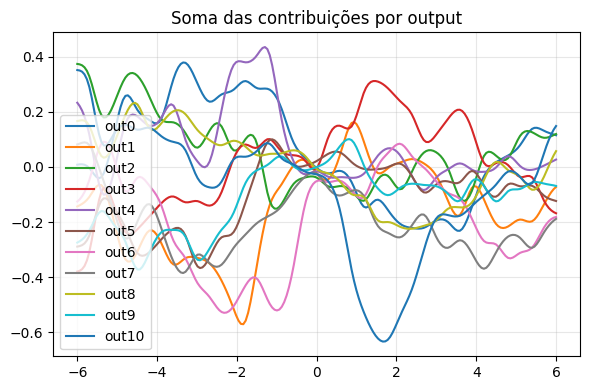
\includegraphics[width=0.28\linewidth]{../output40-66Radam.png} &
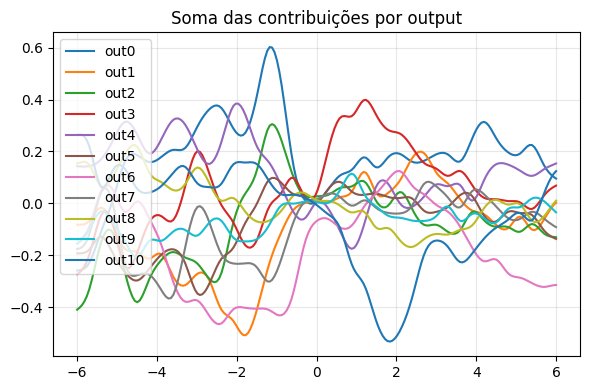
\includegraphics[width=0.28\linewidth]{../output40-66Radamsplineaux.png} & \\
\tiny Grid 40 Clamp-6/6 RAdam &
\tiny Grid 40 Clamp-6/6 RAdam + AuxSpline &
 \\
\end{tabular}
\end{frame}

\section{Conclusões}
\begin{frame}{Conclusões}
\begin{itemize}
\item O seqKAN apresentou desempenho consistente nas métricas globais.
\item Diferença de erro entre grupos indica desbalanceamento forte, pois a série apresenta poucos casos de falhas.
\end{itemize}
\end{frame}

\begin{frame}{Próximos Passos}
\begin{itemize}
\item Comparar com GRU/LSTM/BiLSTM com o mesmo protocolo.
\item Testar variações de grid e regularização no KAN.
\item Incluir gráficos de curvas das splines e ablação.
\end{itemize}
\end{frame}

\end{document}
